\documentclass[letterpaper,10pt,titlepage,draftclsnofoot,onecolumn]{article}

\usepackage{graphicx}                                        
\usepackage{amssymb}                                         
\usepackage{amsmath}                                         
\usepackage{amsthm}                                          

\usepackage{alltt}                                           
\usepackage{float}
\usepackage{color}
\usepackage{url}
\usepackage{hyperref}
\usepackage{listings}

\usepackage{longtable}
\usepackage{balance}
\usepackage[TABBOTCAP, tight]{subfigure}
\usepackage{enumitem}
\usepackage{pstricks, pst-node}

\usepackage{geometry}
\geometry{textheight=8.5in, textwidth=6in}

%random comment

\newcommand{\cred}[1]{{\color{red}#1}}
\newcommand{\cblue}[1]{{\color{blue}#1}}

\newcommand{\toc}{\tableofcontents}

\def\name{Morgan Patch, Mark Bereza}
\def\subj{CS 444 Project 2: I/O Elevators}

%pull in the necessary preamble matter for pygments output
\input{pygments.tex}

% The following metadata will show up in the PDF properties
\hypersetup{
    colorlinks = false,
    urlcolor = black,
    pdfauthor = {\name},
    pdfkeywords = {cs444 ``operating systems'' kernel linux emulator},
    pdftitle = {\subj},
    pdfsubject = {CS 444 Project 2},
    pdfpagemode = UseNone
}

\parindent = 0.0 in
\parskip = 0.1 in

\begin{document}

\begin{titlepage}
	\centering
	{\scshape\huge \subj \par}
	\vspace{1.5cm}
	{\LARGE\bfseries \name\par}

	\vfill
	
	{\large\bfseries Abstract\par}
	\vspace{0.5cm}
	
	For the second project of the course, we implemented a C-LOOK elevator
	as a new I/O scheduler in the Linux kernel, then rebuilt the kernel
	and ran our emulator with the new elevator.
	
	\vfill

    % Bottom of the page
	{\large \today\par}
\end{titlepage}

\tableofcontents
\newpage

\section{Design}

    Implementing the C-LOOK algorithm was rather simple, and mostly required
setting up the elevator\_add\_req\_fn to set up the dispatch queue in the
correct ordering.

    In the noop algorithm, a queue of processed requests ready to be dispatched
is maintained, with new requests pushed to the end of the queue and the
dispatch\_fn pulling off of the front. For our algorithm, the only change we
made to the dispatch function was having it keep track of the head's location
after every dispatch. The real implementation logic for the C-LOOK algorithm was
placed in the add request function. The add function maintains the order of the
queue by placing the items into ascending sort order with the smallest value
following the largest value. For example, if the head is on sector 50, the list
of start sectors of requests in the queue may be:

[58, 82, 90, 104, 123, 168, 177, 13, 22, 38, 41]

    For convenience, I will refer to a request's starting sector location as its
"sect". To achieve the desired ordering, the function first checks to see if the
incoming request has a starting sector location that is greater than or equal to
the current head location:

If it is, the function searches forward until it finds a request with a sect 
greater than the incoming request's sect and places the incoming request right
before it in the queue. To handle the case where there is no request with a
larger sect, a check is done to see where the list "flips"; if the incoming
request's sect is greater than the one's right before the flip, it is placed in
between the requests on either side of the flip.

If the new request's sect is smaller than the current head location, then the
function searches the queue in reverse order until it finds a request with a
sect smaller than the incoming request's and place it right after. To handle the
case where there is no request with a smaller sect, a check is done to see where
the list "flips"; if the incoming request's sect is smaller than the one's right
after the flip, it is placed in between the requests on either side of the flip.

This algorithm, as is, addresses the majority of operations correctly, but two
additional edge cases must be accounted for. The first is when the list is
empty, in which case the incoming request is placed right after the head. The
second is when the current queue consists of a single item whose sect is equal
to the current head location. In this case, there is no identifiable "flip",
so the while loops used to implement the linear searches mentioned earlier never
break. In this case, we simply place the incoming request after the single
request in the queue. This is because no matter what the sect of the incoming
request is, it is correct to first process the request whose sect is right at
the head's location (the one already in the queue).

\section{Questions}

\subsection{What do you think the main point of this assignment is?}

    The point of this assignment seems to be three-fold:
\begin{enumerate}
\item The first point is to learn about block I/O and how its handled in the Linux
kernel. This is a major topic of the class, and it's important for us to
understand how the kernel works and how I/O is scheduled.   

\item The second point is to learn how to make changes to the Linux kernel
without breaking it, and to demystify kernel development to an extent by
encouraging us to dive in headfirst. The Linux kernel is large and unwieldy,
and rather unlike any other kind of C development. It has its own libraries and
patterns and ways to solve problems, and can be extremely intimidating for
people who are new to it. By asking us make a single, modular change to the
kernel, the assignment allows us to dip our toes, so to speak.

\item The third point is to gain experience in beginning development on a large
codebase which has limited, non-existent, hard to locate, or simply incorrect
documentation. In these cases, one has be resourceful in locating the
documentation that does exist and able to do some reverse engineering or pattern
recognition on related source code to determine how the API actually works. In
particular, the asignment description of a similar CS411 assignment from 2011
and the source code for the deadline scheduler proved valuable resources for
understanding to how start the assignment.
\end{enumerate}

\subsection{How did you personally approach the problem?}

    We began by deciding whether to use LOOK or C-LOOK; C-LOOK seemed like the
cleaner solution, and it was a more fair algorithm anyway.

    Next, we used a whiteboard to sketch out the state of the elevator queue
as various requests are added and dispatched; this allowed us to discover the
way to add requests to the queue so that dispatching can just grab the top
request and perform minimal processing. With each change to the algorithm, we
walked through a set of edge cases to ensure that they were being handled
correctly. In particular, we checked for incoming requests larger than any
existing request, incoming requests smaller than any existing request, adding a
request to the empty queue, and handling of requests with identical starting
sectors.

    Then, we implemented our whiteboard psuedocode in actual C code and walked
through the same test cases until we were convined the code would function as
designed.

    Finally, we built the kernel with our custom I/O scheduler, configured the
kernel and QEMU to use it as the default scheduler, and ran QEMU without the
virtio option. The first few times the kernel either crashed or hanged, so we
connected GDB to the QEMU process and set hardware breakpoints inside our add
and dispatch functions and query the state of local variables. To faciliate this
debugging process, printk statement were also placed in the add and dispatch
functions to output the sectors of the each request and some of the local
variables were marked as volatile until debugging we complete to ensure that the
compiler did not optimize them out.

    The debugging process continued until QEMU would boot up and perform basic
I/O operations without any hiccoughs.

\subsection{How did you ensure your solution was correct?}

    First, we manually walked ourselves through our add function as though we
were the computer, with a number of states of the queue and new requests to
add, and confirmed that the function was, in fact, correct. We also confirmed
this way that dispatch could, in fact, always just use the top request.

    We also used `printk` function calls in the various functions, to ensure
that the functions were being called correctly, and that the state of the
elevator queue was accurate.

    Once we were confident our code was correct, we stored a log of the kernel
messages and looked for a series of adds before dispatches to verify that our
elevator was functioning correctly. Here is a useful snippet, for example:

\begin{minipage}{\linewidth}
\begin{center}
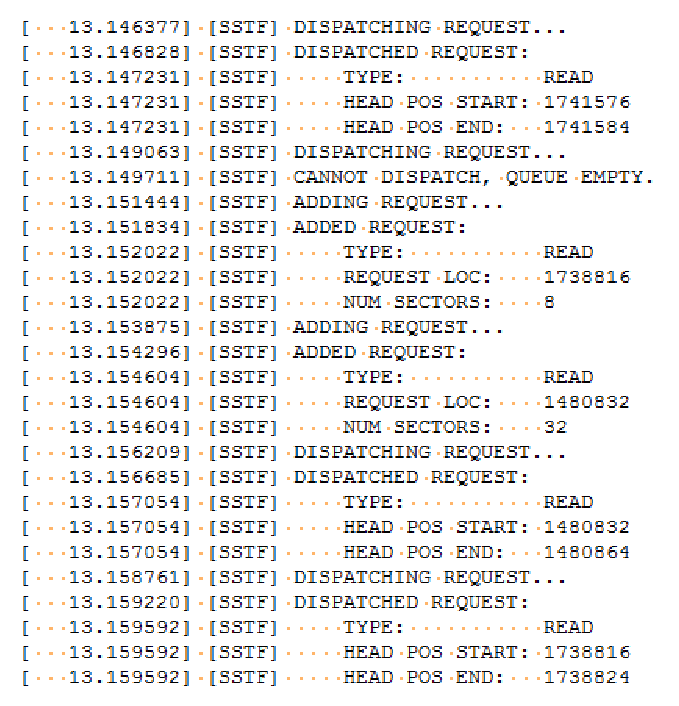
\includegraphics[width=0.6\textwidth]{output_snippet.eps}
\end{center}
\end{minipage}
\\ \\ As you can see, the head is at position 1741584 before the any new
requests are added to the queue. Since we get the "CANNOT DISPACTH, QUEUE EMPTY"
message, we know that the two following requests are the only requests in the
queue. If this elevator were a no-op, it would simply dispatch the requests in
the same order they came in. If it were a LOOK scheduler, it would also process
the first incoming request (1738816) first because it is closer to the current
head's position (1741584). However, since our elevator is a functioning C-LOOK
elevator,it always processes queued requests from smallest to largest (by sector
location), which is exactly what the dispatch messages show.

Finally, we created a Python script that would randomly shuffle files in usr/lib
and then perform a bunch of read/writes to/from these files. We then logged the
printk output to a text file, parsed it for dispatch write sector values and
created a graph from the data:\\
\begin{minipage}{\linewidth}
\begin{center}
\includegraphics[width=\textwidth]{graph.eps}
\end{center}
\end{minipage}
\\ \\As you can see, the dispatches follow a very clean pattern. The first
request is relatively high and the requests are dispatched in increasing order
until the largest request is processed. Then, the dispatches start from the
lowest request and continues steadily foward in sectors for the remaining
dispatches, never once jumping back down during this segment. In this way, it is
clear that our elevator properly functions as a CLOOK evelator.

\subsection{What did you learn?}
By doing this assignment, we learned several things:
\begin{enumerate}
\item We learned how to locate resources for Linux kernel source code. In
particular, the Free Electrons site was very helpful in finding the definitions
of various structs, macros, and functions.
\item We also learned how to use CTags in combination with Emacs to achieve
functionality similar to IntelliSense for the Linux kernel.
\item We learned how to create and apply a patch file using the difference
between two Git repos/branches.
\item We learned how to make QEMU use a regular drive format vs virtio.
\item We learned how to configure certain kernel settings; specifically, how to
change the default scheduler.
\item We learned the differences between some of the common I/O scheduling
algorithms.
\end{enumerate}

\subsection{How should the TA evaluate your work?}
In order to evaluate our work, the TA should take the following steps:
\begin{enumerate}
\item Examine our source code, provided below, to see if our approach to the add
request function makes sense.
\item Examine the snippet and graphs provided in this writeup and verify that
the data matches how a CLOOK I/O scheduler should operate.
\item Clone the linux yocto repository:\\
\texttt{git clone git://git.yoctoproject.org/linux-yocto-3.19}
\item Switch to the v3.19.2 tag:\\
\texttt{cd linux-yocto-3.19/} \\
\texttt{git checkout tags/v3.19.2}
\item Apply the patch file provided with this submission:\\
\texttt{git apply assignment2.patch}
\item Copy the configuration file from scratch:\\
\texttt{cp /scratch/files/config-3.19.2-yocto-standard ./.config}
\item Copy the core image file from scratch:\\
\texttt{cp /scratch/files/core-image-lsb-sdk-qemux86.ext4 .}
\item Setup environment variables:\\
\texttt{source /scratch/files/environment-setup-i586-poky-linux} (if using bash/zsh) \\
OR \\
\texttt{source /scratch/files/environment-setup-i586-poky-linux.csh} (if using tcsh/csh)
\item Edit the configuration to use our scheduler:\\
\texttt{make menuconfig} \\
Then go to Enable the block layer$\rightarrow$IO schedulers$\rightarrow$Default IO scheduler$\rightarrow$select "SSTF"\\
Save this configuration to .config and exit menuconfig.
\item Build the kernel:\\
\texttt{make all -j4}
\item Run the kernel using QEMU:\\
\texttt{qemu-system-i386 -nographic -kernel arch/x86/boot/bzImage -drive file=core-image-lsb-sdk-qemux86.ext4 -enable-kvm -net none -usb -localtime --no-reboot --append "root=/dev/hda rw console=ttyS0 debug elevator=sstf"}
\item Verify that the kernel boots and you can login to root.
\item The kernel will be printing a massive amount of messages regarding requests being added and dispatched. Make sure that this output follows what a CLOOK I/O scheduler should be doing.
\item If you wish to be super sure, feel free to run the Python script included with this file on the emulated machine. Then, you can save the kernel output produced during the running of said script using:\\
\texttt{dmesg | grep SSTF > sstf.txt}\\
If you open this file and scroll until you see the writes, you will get a nice number of adds followed by a nice number of dispatches. This is the data that was used to generate our graph. You can visually verify that requests are being dispatched from lowest to highest sector with the exception of when the highest sector request is dispatched, after which the next request will be the lowest in the queue. To see an example of such an output without having to run the Python script yourself, simply refer to the sstf-write.txt file included with this submission.
\end{enumerate}

\section{Version Control Log}

%% This file was generated by the script latex-git-log
\begin{tabular}{lp{8cm}}
  \label{tabular:legend:git-log}
  \textbf{acronym} & \textbf{meaning} \\
  V & \texttt{version} \\
  tag & \texttt{git tag} \\
  MF & Number of \texttt{modified files}. \\
  AL & Number of \texttt{added lines}. \\
  DL & Number of \texttt{deleted lines}. \\
\end{tabular}

\bigskip

\iflanguage{ngerman}{\shorthandoff{"}}{}
\begin{longtable}{|rlllrrr|}
\hline \multicolumn{1}{|c}{\textbf{V}} & \multicolumn{1}{c}{\textbf{tag}}
& \multicolumn{1}{c}{\textbf{date}}
& \multicolumn{1}{c}{\textbf{commit message}} & \multicolumn{1}{c}{\textbf{MF}}
& \multicolumn{1}{c}{\textbf{AL}} & \multicolumn{1}{c|}{\textbf{DL}} \\ \hline
\endhead

\hline \multicolumn{7}{|r|}{} \\ \hline
\endfoot

\hline% \hline
\endlastfoot

\hline 1 &  & 2017-10-19 & Add Linux Yocto at tag 3.19.2. & 48441 & 19142068 & 0 \\
\hline 2 &  & 2017-10-19 & Add blank LOOK file. & 1 & 0 & 0 \\
\hline 3 &  & 2017-10-28 & Copy noop to c-look scheduler. & 1 & 124 & 0 \\
\hline 4 &  & 2017-10-28 & Setup elevator configuration in preparation for code. & 3 & 15 & 2 \\
\hline 5 &  & 2017-10-28 & Add finished add\_request function. & 1 & 19 & 2 \\
\hline 6 &  & 2017-10-28 & Remove unnecessary while loop. & 1 & 5 & 8 \\
\hline 7 &  & 2017-10-29 & Add latter and former functions. & 3 & 7 & 6 \\
\hline 8 &  & 2017-10-30 & Add line to skip sentinel in add, make former like latter. & 1 & 4 & 2 \\
\hline 9 &  & 2017-10-30 & Fix a few typos. & 2 & 2 & 2 \\
\hline 10 &  & 2017-10-30 & Naming changes and added printks & 3 & 20 & 21 \\
\hline 11 &  & 2017-10-30 & naming changes and improved printk messages & 1 & 50 & 32 \\
\hline 12 &  & 2017-10-30 & writeup: Write preliminary design section and work log. & 3 & 627 & 0 \\
\hline 13 &  & 2017-10-30 & Fixed add\_request() algorithm and indenting & 1 & 113 & 92 \\
\hline 14 &  & 2017-10-30 & writeup: Add question 1. & 1 & 18 & 324 \\
\hline 15 &  & 2017-10-30 & writeup: Write next 2 questions. & 1 & 22 & 0 \\
\hline 16 &  & 2017-10-30 & Fixed formatting of printk statements & 1 & 15 & 15 \\
\hline 17 &  & 2017-10-30 & Fixed printk messages and whitespace & 1 & 35 & 32 \\
\hline 18 &  & 2017-10-30 & Fixed add\_request when request is smaller than head\_loc & 1 & 26 & 9 \\
\hline 19 &  & 2017-10-30 & Fixed case where single item with sect same as head\_loc & 1 & 5 & 3 \\
\hline 20 &  & 2017-10-30 & whitespace change & 1 & 1 & 1 \\
\hline 21 &  & 2017-10-30 & First three sections of writeup, minor corrections & 1 & 67 & 21 \\
\hline 22 &  & 2017-10-30 & More changes to writeup, include output and code & 4 & 14210 & 22 \\
\hline 23 &  & 2017-10-30 & Almost done with writeup & 2 & 94328 & 0 \\
\hline 24 &  & 2017-10-30 & Add version control log. & 2 & 259 & 202 \\
\end{longtable}

\section{Work Log}

\begin{itemize}
    \item Friday, 2017-10-27
    
        \begin{itemize}
            \item Looked over assignment description.
        \end{itemize}
    
    \item Saturday, 2017-10-28
    
        \begin{itemize}
            \item Planned our solution on whiteboards.
            \item Researched elevator algorithms.
            \item Agreed to write C-LOOK.
            \item Wrote the add\_request\_fn, confirmed it worked.
            \item Spent a lot of time building the kernel.
            \item Added our elevator to the kernel configuration.
            \item Fixed some issues with our configuration.
        \end{itemize}
        
    \item Sunday, 2017-10-29
    
        \begin{itemize}
            \item Wrote the former\_req\_fn and latter\_req\_fn.
            \item Confirmed that our dispatch function was correct.
            \item Researched how merges work.
            \item Accidentally broke our kernel config, spent a lot of time fixing that.
            \item Began working on some parts of writeup.
        \end{itemize}
        
    \item Monday, 2017-10-30
    
        \begin{itemize}
            \item Added work log and Design sections to writeup.
			\item Played with QEMU settings until it ran successfully without virtio.
			\item Fixed algorithm to address a few unnoticed corner cases.
			\item Inspected dmesg output to ensure that the elevator was functioning correctly.
			\item Wrote a script to exercise I/O and plotted the dispatch sectors.
			\item Finalized writeup.
        \end{itemize}
\end{itemize}

\section*{Appendix 1: Source Code}
\subsection{sstf-iosched.c}

\lstset{language=C}

\begin{lstlisting}
/*
* elevator C-LOOK
*/
#include <linux/blkdev.h>
#include <linux/elevator.h>
#include <linux/bio.h>
#include <linux/module.h>
#include <linux/slab.h>
#include <linux/init.h>

#define get_sector(X) blk_rq_pos(list_entry(X, struct request, queuelist))

struct sstf_data {
        struct list_head queue;
        sector_t head_loc;
};

static void sstf_merged_requests(struct request_queue *q,
                                 struct request *rq,
                                 struct request *next)
{
        list_del_init(&next->queuelist);
}

static int sstf_dispatch(struct request_queue *q, int force)
{
        struct sstf_data *nd = q->elevator->elevator_data;

        printk("[SSTF] DISPATCHING REQUEST...\n");

        if (!list_empty(&(nd->queue))) {
                struct request *rq;
                rq = list_entry(nd->queue.next, struct request, queuelist);
                list_del_init(&(rq->queuelist));
                elv_dispatch_sort(q, rq);
                nd->head_loc = rq_end_sector(rq);

                printk("[SSTF] DISPATCHED REQUEST:\n");
                if (rq_data_dir(rq) == READ) {
                        printk("[SSTF]     TYPE:           READ\n");
                }
                else {
                        printk("[SSTF]     TYPE:           WRITE\n");
                }
                printk("[SSTF]     HEAD POS START: %lu\n", blk_rq_pos(rq));
                printk("[SSTF]     HEAD POS END:   %lu\n", rq_end_sector(rq));
                
                return 1;
        }

        printk("[SSTF] CANNOT DISPATCH, QUEUE EMPTY.\n");
        return 0;
}

static void sstf_add_request(struct request_queue *q, struct request *rq)
{
        struct sstf_data *nd = q->elevator->elevator_data;
        struct list_head *cur = &(nd->queue);

        printk("[SSTF] ADDING REQUEST...\n");

        if (!list_empty(&nd->queue)) {
                struct list_head *next = cur->next;
                sector_t cur_sect  = nd->head_loc;
                sector_t next_sect = get_sector(next);
                sector_t rq_sect   = blk_rq_pos(rq);
                if ((cur->next == cur->prev) && (cur_sect == next_sect)) {
                        cur = cur->next;
                } else if (rq_sect < nd->head_loc) {
                        while (rq_sect < cur_sect) {
                                if ((cur_sect > next_sect) &&
                                    (rq_sect < next_sect)) {
                                        break;
                                }
                                next = cur;
                                next_sect = cur_sect;
                                cur = cur->prev;
                                cur_sect = (cur == &(nd->queue)) ?
                                           nd->head_loc          :
                                           get_sector(cur);
                        }
                } else {
                        while (next_sect < rq_sect) {
                                if ((cur_sect > next_sect) && 
                                    (rq_sect > cur_sect)) {
                                        break;
                                }
                                cur = next;
                                cur_sect = next_sect;
                                next = next->next;
                                next_sect = (next == &(nd->queue)) ?
                                        nd->head_loc               :
                                        get_sector(next);
                        }
                }
                
        }
        list_add(&(rq->queuelist), cur);

        printk("[SSTF] ADDED REQUEST:\n");
        if (rq_data_dir(rq) == READ) {
                printk("[SSTF]     TYPE:           READ\n");
        }
        else {
                printk("[SSTF]     TYPE:           WRITE\n");
        }
        printk("[SSTF]     REQUEST LOC:    %lu\n", blk_rq_pos(rq));
        printk("[SSTF]     NUM SECTORS:    %lu\n", blk_rq_sectors(rq));
}

static struct request *
sstf_former_request(struct request_queue *q, struct request *rq)
{
        struct sstf_data *nd = q->elevator->elevator_data;

        if (list_empty(&nd->queue))
                return NULL;
        return list_entry(nd->queue.prev, struct request, queuelist);
}

static struct request *
sstf_latter_request(struct request_queue *q, struct request *rq)
{
        struct sstf_data *nd = q->elevator->elevator_data;

        if (list_empty(&nd->queue))
                return NULL;
        return list_entry(nd->queue.next, struct request, queuelist);
}

static int sstf_init_queue(struct request_queue *q, struct elevator_type *e)
{
        struct sstf_data *nd;
        struct elevator_queue *eq;

        printk("[SSTF] INITIALIZING...\n");
        
        eq = elevator_alloc(q, e);
        if (!eq)
                return -ENOMEM;

        nd = kmalloc_node(sizeof(*nd), GFP_KERNEL, q->node);
        if (!nd) {
                kobject_put(&eq->kobj);
                return -ENOMEM;
        }
        eq->elevator_data = nd;

        INIT_LIST_HEAD(&nd->queue);
        nd->head_loc = 0;

        spin_lock_irq(q->queue_lock);
        q->elevator = eq;
        spin_unlock_irq(q->queue_lock);

        printk("[SSTF] INITIALIZED\n");
        return 0;
}

static void sstf_exit_queue(struct elevator_queue *e)
{
        struct sstf_data *nd = e->elevator_data;

        printk("[SSTF] EXITING...\n");

        BUG_ON(!list_empty(&nd->queue));
        kfree(nd);

        printk("[SSTF] EXITED\n");
}

static struct elevator_type elevator_sstf = {
        .ops = {
                .elevator_merge_req_fn  = sstf_merged_requests,
                .elevator_dispatch_fn   = sstf_dispatch,
                .elevator_add_req_fn    = sstf_add_request,
                .elevator_former_req_fn = sstf_former_request,
                .elevator_latter_req_fn = sstf_latter_request,
                .elevator_init_fn       = sstf_init_queue,
                .elevator_exit_fn       = sstf_exit_queue,
         },
        .elevator_name = "sstf",
        .elevator_owner = THIS_MODULE,
};

static int __init sstf_init(void)
{
        return elv_register(&elevator_sstf);
}

static void __exit sstf_exit(void)
{
        elv_unregister(&elevator_sstf);
}

module_init(sstf_init);
module_exit(sstf_exit);

MODULE_AUTHOR("Morgan Patch / Mark Bereza");
MODULE_LICENSE("GPL");
MODULE_DESCRIPTION("SSTF IO scheduler");
\end{lstlisting}

\end{document}
